Finally, we performed the same prediction tasks ask before, for wind energy.
Figure \ref{fig:wind48} and Figure \ref{fig:wind04} show the best forecasts
that minimized the RMSE for
48 and 4-hours ahead, respectively. All features except air pressure improved
the forecast. Including solar elevation angle improved the 48-hour ahead
forecast the most, while adding windspeed improved the 4-hour ahead the most.
Those results are shown in Table \ref{tab:wind48} and \ref{tab:wind04}
respectively. Qualitatively, our conventional \gls{esn} achieved results
comparable to a more complex algorithm by simply adding a single meteorological
predictor \cite{lopez_wind_2018}. The results for a 48-hour ahead forecast from
a more complex algorithm are shown in Figure \ref{fig:lopez2018}.

However, the state-of-the-art Weather Research and Forecasting model
\cite{powers_weather_2017}, a numerical weather prediction model, far
outperforms our best results. Thus, conventional \glspl{esn} are insufficient
for applications in grid planning \cite{wang_quantifying_2016}.

\begin{figure*}[h]
  \centering
  % 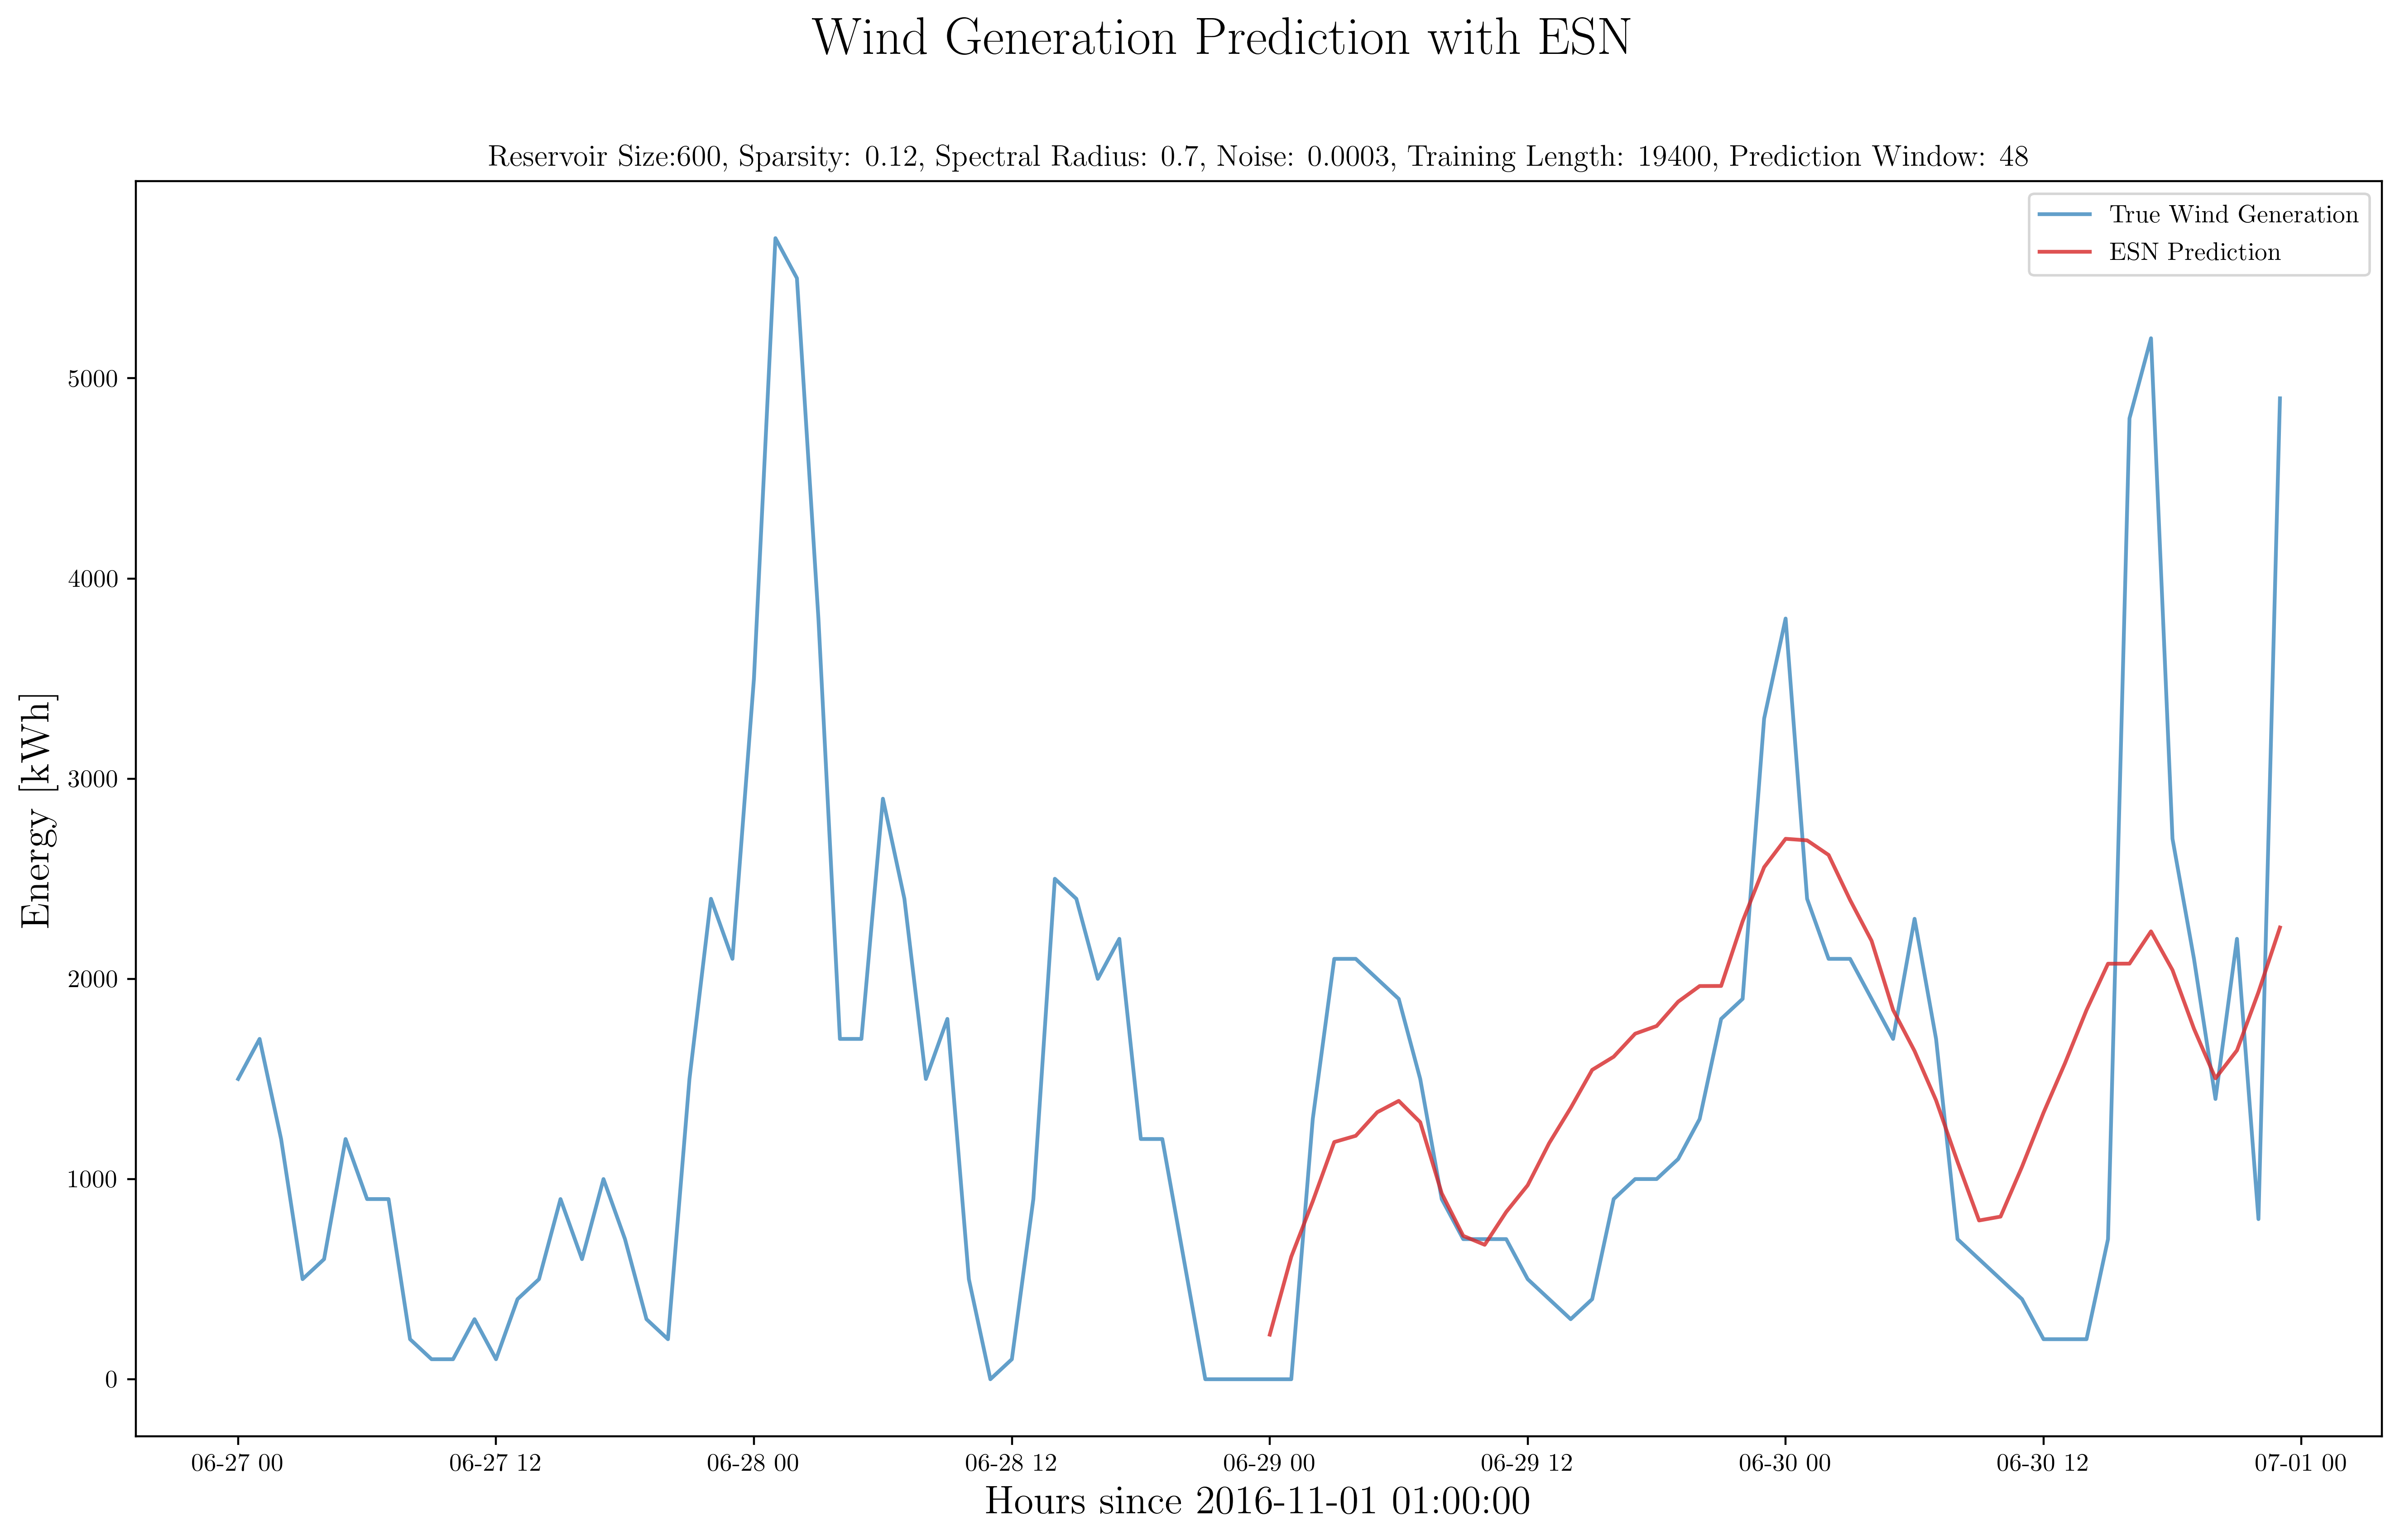
\includegraphics[width=0.8\textwidth]{48_wind_elevation_prediction.png}
  %% Creator: Matplotlib, PGF backend
%%
%% To include the figure in your LaTeX document, write
%%   \input{<filename>.pgf}
%%
%% Make sure the required packages are loaded in your preamble
%%   \usepackage{pgf}
%%
%% Figures using additional raster images can only be included by \input if
%% they are in the same directory as the main LaTeX file. For loading figures
%% from other directories you can use the `import` package
%%   \usepackage{import}
%% and then include the figures with
%%   \import{<path to file>}{<filename>.pgf}
%%
%% Matplotlib used the following preamble
%%
\begingroup%
\makeatletter%
\begin{pgfpicture}%
\pgfpathrectangle{\pgfpointorigin}{\pgfqpoint{5.531696in}{3.164528in}}%
\pgfusepath{use as bounding box, clip}%
\begin{pgfscope}%
\pgfsetbuttcap%
\pgfsetmiterjoin%
\definecolor{currentfill}{rgb}{1.000000,1.000000,1.000000}%
\pgfsetfillcolor{currentfill}%
\pgfsetlinewidth{0.000000pt}%
\definecolor{currentstroke}{rgb}{1.000000,1.000000,1.000000}%
\pgfsetstrokecolor{currentstroke}%
\pgfsetdash{}{0pt}%
\pgfpathmoveto{\pgfqpoint{0.000000in}{0.000000in}}%
\pgfpathlineto{\pgfqpoint{5.531696in}{0.000000in}}%
\pgfpathlineto{\pgfqpoint{5.531696in}{3.164528in}}%
\pgfpathlineto{\pgfqpoint{0.000000in}{3.164528in}}%
\pgfpathclose%
\pgfusepath{fill}%
\end{pgfscope}%
\begin{pgfscope}%
\pgfsetbuttcap%
\pgfsetmiterjoin%
\definecolor{currentfill}{rgb}{1.000000,1.000000,1.000000}%
\pgfsetfillcolor{currentfill}%
\pgfsetlinewidth{0.000000pt}%
\definecolor{currentstroke}{rgb}{0.000000,0.000000,0.000000}%
\pgfsetstrokecolor{currentstroke}%
\pgfsetstrokeopacity{0.000000}%
\pgfsetdash{}{0pt}%
\pgfpathmoveto{\pgfqpoint{0.669445in}{0.499691in}}%
\pgfpathlineto{\pgfqpoint{5.431696in}{0.499691in}}%
\pgfpathlineto{\pgfqpoint{5.431696in}{2.865455in}}%
\pgfpathlineto{\pgfqpoint{0.669445in}{2.865455in}}%
\pgfpathclose%
\pgfusepath{fill}%
\end{pgfscope}%
\begin{pgfscope}%
\pgfsetbuttcap%
\pgfsetroundjoin%
\definecolor{currentfill}{rgb}{0.000000,0.000000,0.000000}%
\pgfsetfillcolor{currentfill}%
\pgfsetlinewidth{0.803000pt}%
\definecolor{currentstroke}{rgb}{0.000000,0.000000,0.000000}%
\pgfsetstrokecolor{currentstroke}%
\pgfsetdash{}{0pt}%
\pgfsys@defobject{currentmarker}{\pgfqpoint{0.000000in}{-0.048611in}}{\pgfqpoint{0.000000in}{0.000000in}}{%
\pgfpathmoveto{\pgfqpoint{0.000000in}{0.000000in}}%
\pgfpathlineto{\pgfqpoint{0.000000in}{-0.048611in}}%
\pgfusepath{stroke,fill}%
}%
\begin{pgfscope}%
\pgfsys@transformshift{1.250485in}{0.499691in}%
\pgfsys@useobject{currentmarker}{}%
\end{pgfscope}%
\end{pgfscope}%
\begin{pgfscope}%
\definecolor{textcolor}{rgb}{0.000000,0.000000,0.000000}%
\pgfsetstrokecolor{textcolor}%
\pgfsetfillcolor{textcolor}%
\pgftext[x=1.250485in,y=0.402469in,,top]{\color{textcolor}\rmfamily\fontsize{10.000000}{12.000000}\selectfont \(\displaystyle 23240\)}%
\end{pgfscope}%
\begin{pgfscope}%
\pgfsetbuttcap%
\pgfsetroundjoin%
\definecolor{currentfill}{rgb}{0.000000,0.000000,0.000000}%
\pgfsetfillcolor{currentfill}%
\pgfsetlinewidth{0.803000pt}%
\definecolor{currentstroke}{rgb}{0.000000,0.000000,0.000000}%
\pgfsetstrokecolor{currentstroke}%
\pgfsetdash{}{0pt}%
\pgfsys@defobject{currentmarker}{\pgfqpoint{0.000000in}{-0.048611in}}{\pgfqpoint{0.000000in}{0.000000in}}{%
\pgfpathmoveto{\pgfqpoint{0.000000in}{0.000000in}}%
\pgfpathlineto{\pgfqpoint{0.000000in}{-0.048611in}}%
\pgfusepath{stroke,fill}%
}%
\begin{pgfscope}%
\pgfsys@transformshift{2.161921in}{0.499691in}%
\pgfsys@useobject{currentmarker}{}%
\end{pgfscope}%
\end{pgfscope}%
\begin{pgfscope}%
\definecolor{textcolor}{rgb}{0.000000,0.000000,0.000000}%
\pgfsetstrokecolor{textcolor}%
\pgfsetfillcolor{textcolor}%
\pgftext[x=2.161921in,y=0.402469in,,top]{\color{textcolor}\rmfamily\fontsize{10.000000}{12.000000}\selectfont \(\displaystyle 23260\)}%
\end{pgfscope}%
\begin{pgfscope}%
\pgfsetbuttcap%
\pgfsetroundjoin%
\definecolor{currentfill}{rgb}{0.000000,0.000000,0.000000}%
\pgfsetfillcolor{currentfill}%
\pgfsetlinewidth{0.803000pt}%
\definecolor{currentstroke}{rgb}{0.000000,0.000000,0.000000}%
\pgfsetstrokecolor{currentstroke}%
\pgfsetdash{}{0pt}%
\pgfsys@defobject{currentmarker}{\pgfqpoint{0.000000in}{-0.048611in}}{\pgfqpoint{0.000000in}{0.000000in}}{%
\pgfpathmoveto{\pgfqpoint{0.000000in}{0.000000in}}%
\pgfpathlineto{\pgfqpoint{0.000000in}{-0.048611in}}%
\pgfusepath{stroke,fill}%
}%
\begin{pgfscope}%
\pgfsys@transformshift{3.073357in}{0.499691in}%
\pgfsys@useobject{currentmarker}{}%
\end{pgfscope}%
\end{pgfscope}%
\begin{pgfscope}%
\definecolor{textcolor}{rgb}{0.000000,0.000000,0.000000}%
\pgfsetstrokecolor{textcolor}%
\pgfsetfillcolor{textcolor}%
\pgftext[x=3.073357in,y=0.402469in,,top]{\color{textcolor}\rmfamily\fontsize{10.000000}{12.000000}\selectfont \(\displaystyle 23280\)}%
\end{pgfscope}%
\begin{pgfscope}%
\pgfsetbuttcap%
\pgfsetroundjoin%
\definecolor{currentfill}{rgb}{0.000000,0.000000,0.000000}%
\pgfsetfillcolor{currentfill}%
\pgfsetlinewidth{0.803000pt}%
\definecolor{currentstroke}{rgb}{0.000000,0.000000,0.000000}%
\pgfsetstrokecolor{currentstroke}%
\pgfsetdash{}{0pt}%
\pgfsys@defobject{currentmarker}{\pgfqpoint{0.000000in}{-0.048611in}}{\pgfqpoint{0.000000in}{0.000000in}}{%
\pgfpathmoveto{\pgfqpoint{0.000000in}{0.000000in}}%
\pgfpathlineto{\pgfqpoint{0.000000in}{-0.048611in}}%
\pgfusepath{stroke,fill}%
}%
\begin{pgfscope}%
\pgfsys@transformshift{3.984792in}{0.499691in}%
\pgfsys@useobject{currentmarker}{}%
\end{pgfscope}%
\end{pgfscope}%
\begin{pgfscope}%
\definecolor{textcolor}{rgb}{0.000000,0.000000,0.000000}%
\pgfsetstrokecolor{textcolor}%
\pgfsetfillcolor{textcolor}%
\pgftext[x=3.984792in,y=0.402469in,,top]{\color{textcolor}\rmfamily\fontsize{10.000000}{12.000000}\selectfont \(\displaystyle 23300\)}%
\end{pgfscope}%
\begin{pgfscope}%
\pgfsetbuttcap%
\pgfsetroundjoin%
\definecolor{currentfill}{rgb}{0.000000,0.000000,0.000000}%
\pgfsetfillcolor{currentfill}%
\pgfsetlinewidth{0.803000pt}%
\definecolor{currentstroke}{rgb}{0.000000,0.000000,0.000000}%
\pgfsetstrokecolor{currentstroke}%
\pgfsetdash{}{0pt}%
\pgfsys@defobject{currentmarker}{\pgfqpoint{0.000000in}{-0.048611in}}{\pgfqpoint{0.000000in}{0.000000in}}{%
\pgfpathmoveto{\pgfqpoint{0.000000in}{0.000000in}}%
\pgfpathlineto{\pgfqpoint{0.000000in}{-0.048611in}}%
\pgfusepath{stroke,fill}%
}%
\begin{pgfscope}%
\pgfsys@transformshift{4.896228in}{0.499691in}%
\pgfsys@useobject{currentmarker}{}%
\end{pgfscope}%
\end{pgfscope}%
\begin{pgfscope}%
\definecolor{textcolor}{rgb}{0.000000,0.000000,0.000000}%
\pgfsetstrokecolor{textcolor}%
\pgfsetfillcolor{textcolor}%
\pgftext[x=4.896228in,y=0.402469in,,top]{\color{textcolor}\rmfamily\fontsize{10.000000}{12.000000}\selectfont \(\displaystyle 23320\)}%
\end{pgfscope}%
\begin{pgfscope}%
\definecolor{textcolor}{rgb}{0.000000,0.000000,0.000000}%
\pgfsetstrokecolor{textcolor}%
\pgfsetfillcolor{textcolor}%
\pgftext[x=3.050571in,y=0.223457in,,top]{\color{textcolor}\rmfamily\fontsize{10.000000}{12.000000}\selectfont Hours since 2016-11-01 01:00:00}%
\end{pgfscope}%
\begin{pgfscope}%
\pgfsetbuttcap%
\pgfsetroundjoin%
\definecolor{currentfill}{rgb}{0.000000,0.000000,0.000000}%
\pgfsetfillcolor{currentfill}%
\pgfsetlinewidth{0.803000pt}%
\definecolor{currentstroke}{rgb}{0.000000,0.000000,0.000000}%
\pgfsetstrokecolor{currentstroke}%
\pgfsetdash{}{0pt}%
\pgfsys@defobject{currentmarker}{\pgfqpoint{-0.048611in}{0.000000in}}{\pgfqpoint{0.000000in}{0.000000in}}{%
\pgfpathmoveto{\pgfqpoint{0.000000in}{0.000000in}}%
\pgfpathlineto{\pgfqpoint{-0.048611in}{0.000000in}}%
\pgfusepath{stroke,fill}%
}%
\begin{pgfscope}%
\pgfsys@transformshift{0.669445in}{0.607226in}%
\pgfsys@useobject{currentmarker}{}%
\end{pgfscope}%
\end{pgfscope}%
\begin{pgfscope}%
\definecolor{textcolor}{rgb}{0.000000,0.000000,0.000000}%
\pgfsetstrokecolor{textcolor}%
\pgfsetfillcolor{textcolor}%
\pgftext[x=0.502778in,y=0.559001in,left,base]{\color{textcolor}\rmfamily\fontsize{10.000000}{12.000000}\selectfont \(\displaystyle 0\)}%
\end{pgfscope}%
\begin{pgfscope}%
\pgfsetbuttcap%
\pgfsetroundjoin%
\definecolor{currentfill}{rgb}{0.000000,0.000000,0.000000}%
\pgfsetfillcolor{currentfill}%
\pgfsetlinewidth{0.803000pt}%
\definecolor{currentstroke}{rgb}{0.000000,0.000000,0.000000}%
\pgfsetstrokecolor{currentstroke}%
\pgfsetdash{}{0pt}%
\pgfsys@defobject{currentmarker}{\pgfqpoint{-0.048611in}{0.000000in}}{\pgfqpoint{0.000000in}{0.000000in}}{%
\pgfpathmoveto{\pgfqpoint{0.000000in}{0.000000in}}%
\pgfpathlineto{\pgfqpoint{-0.048611in}{0.000000in}}%
\pgfusepath{stroke,fill}%
}%
\begin{pgfscope}%
\pgfsys@transformshift{0.669445in}{0.984541in}%
\pgfsys@useobject{currentmarker}{}%
\end{pgfscope}%
\end{pgfscope}%
\begin{pgfscope}%
\definecolor{textcolor}{rgb}{0.000000,0.000000,0.000000}%
\pgfsetstrokecolor{textcolor}%
\pgfsetfillcolor{textcolor}%
\pgftext[x=0.294444in,y=0.936315in,left,base]{\color{textcolor}\rmfamily\fontsize{10.000000}{12.000000}\selectfont \(\displaystyle 1000\)}%
\end{pgfscope}%
\begin{pgfscope}%
\pgfsetbuttcap%
\pgfsetroundjoin%
\definecolor{currentfill}{rgb}{0.000000,0.000000,0.000000}%
\pgfsetfillcolor{currentfill}%
\pgfsetlinewidth{0.803000pt}%
\definecolor{currentstroke}{rgb}{0.000000,0.000000,0.000000}%
\pgfsetstrokecolor{currentstroke}%
\pgfsetdash{}{0pt}%
\pgfsys@defobject{currentmarker}{\pgfqpoint{-0.048611in}{0.000000in}}{\pgfqpoint{0.000000in}{0.000000in}}{%
\pgfpathmoveto{\pgfqpoint{0.000000in}{0.000000in}}%
\pgfpathlineto{\pgfqpoint{-0.048611in}{0.000000in}}%
\pgfusepath{stroke,fill}%
}%
\begin{pgfscope}%
\pgfsys@transformshift{0.669445in}{1.361855in}%
\pgfsys@useobject{currentmarker}{}%
\end{pgfscope}%
\end{pgfscope}%
\begin{pgfscope}%
\definecolor{textcolor}{rgb}{0.000000,0.000000,0.000000}%
\pgfsetstrokecolor{textcolor}%
\pgfsetfillcolor{textcolor}%
\pgftext[x=0.294444in,y=1.313630in,left,base]{\color{textcolor}\rmfamily\fontsize{10.000000}{12.000000}\selectfont \(\displaystyle 2000\)}%
\end{pgfscope}%
\begin{pgfscope}%
\pgfsetbuttcap%
\pgfsetroundjoin%
\definecolor{currentfill}{rgb}{0.000000,0.000000,0.000000}%
\pgfsetfillcolor{currentfill}%
\pgfsetlinewidth{0.803000pt}%
\definecolor{currentstroke}{rgb}{0.000000,0.000000,0.000000}%
\pgfsetstrokecolor{currentstroke}%
\pgfsetdash{}{0pt}%
\pgfsys@defobject{currentmarker}{\pgfqpoint{-0.048611in}{0.000000in}}{\pgfqpoint{0.000000in}{0.000000in}}{%
\pgfpathmoveto{\pgfqpoint{0.000000in}{0.000000in}}%
\pgfpathlineto{\pgfqpoint{-0.048611in}{0.000000in}}%
\pgfusepath{stroke,fill}%
}%
\begin{pgfscope}%
\pgfsys@transformshift{0.669445in}{1.739170in}%
\pgfsys@useobject{currentmarker}{}%
\end{pgfscope}%
\end{pgfscope}%
\begin{pgfscope}%
\definecolor{textcolor}{rgb}{0.000000,0.000000,0.000000}%
\pgfsetstrokecolor{textcolor}%
\pgfsetfillcolor{textcolor}%
\pgftext[x=0.294444in,y=1.690945in,left,base]{\color{textcolor}\rmfamily\fontsize{10.000000}{12.000000}\selectfont \(\displaystyle 3000\)}%
\end{pgfscope}%
\begin{pgfscope}%
\pgfsetbuttcap%
\pgfsetroundjoin%
\definecolor{currentfill}{rgb}{0.000000,0.000000,0.000000}%
\pgfsetfillcolor{currentfill}%
\pgfsetlinewidth{0.803000pt}%
\definecolor{currentstroke}{rgb}{0.000000,0.000000,0.000000}%
\pgfsetstrokecolor{currentstroke}%
\pgfsetdash{}{0pt}%
\pgfsys@defobject{currentmarker}{\pgfqpoint{-0.048611in}{0.000000in}}{\pgfqpoint{0.000000in}{0.000000in}}{%
\pgfpathmoveto{\pgfqpoint{0.000000in}{0.000000in}}%
\pgfpathlineto{\pgfqpoint{-0.048611in}{0.000000in}}%
\pgfusepath{stroke,fill}%
}%
\begin{pgfscope}%
\pgfsys@transformshift{0.669445in}{2.116485in}%
\pgfsys@useobject{currentmarker}{}%
\end{pgfscope}%
\end{pgfscope}%
\begin{pgfscope}%
\definecolor{textcolor}{rgb}{0.000000,0.000000,0.000000}%
\pgfsetstrokecolor{textcolor}%
\pgfsetfillcolor{textcolor}%
\pgftext[x=0.294444in,y=2.068259in,left,base]{\color{textcolor}\rmfamily\fontsize{10.000000}{12.000000}\selectfont \(\displaystyle 4000\)}%
\end{pgfscope}%
\begin{pgfscope}%
\pgfsetbuttcap%
\pgfsetroundjoin%
\definecolor{currentfill}{rgb}{0.000000,0.000000,0.000000}%
\pgfsetfillcolor{currentfill}%
\pgfsetlinewidth{0.803000pt}%
\definecolor{currentstroke}{rgb}{0.000000,0.000000,0.000000}%
\pgfsetstrokecolor{currentstroke}%
\pgfsetdash{}{0pt}%
\pgfsys@defobject{currentmarker}{\pgfqpoint{-0.048611in}{0.000000in}}{\pgfqpoint{0.000000in}{0.000000in}}{%
\pgfpathmoveto{\pgfqpoint{0.000000in}{0.000000in}}%
\pgfpathlineto{\pgfqpoint{-0.048611in}{0.000000in}}%
\pgfusepath{stroke,fill}%
}%
\begin{pgfscope}%
\pgfsys@transformshift{0.669445in}{2.493799in}%
\pgfsys@useobject{currentmarker}{}%
\end{pgfscope}%
\end{pgfscope}%
\begin{pgfscope}%
\definecolor{textcolor}{rgb}{0.000000,0.000000,0.000000}%
\pgfsetstrokecolor{textcolor}%
\pgfsetfillcolor{textcolor}%
\pgftext[x=0.294444in,y=2.445574in,left,base]{\color{textcolor}\rmfamily\fontsize{10.000000}{12.000000}\selectfont \(\displaystyle 5000\)}%
\end{pgfscope}%
\begin{pgfscope}%
\definecolor{textcolor}{rgb}{0.000000,0.000000,0.000000}%
\pgfsetstrokecolor{textcolor}%
\pgfsetfillcolor{textcolor}%
\pgftext[x=0.238889in,y=1.682573in,,bottom,rotate=90.000000]{\color{textcolor}\rmfamily\fontsize{10.000000}{12.000000}\selectfont Energy [kWh]}%
\end{pgfscope}%
\begin{pgfscope}%
\pgfpathrectangle{\pgfqpoint{0.669445in}{0.499691in}}{\pgfqpoint{4.762251in}{2.365763in}}%
\pgfusepath{clip}%
\pgfsetrectcap%
\pgfsetroundjoin%
\pgfsetlinewidth{1.505625pt}%
\definecolor{currentstroke}{rgb}{0.121569,0.466667,0.705882}%
\pgfsetstrokecolor{currentstroke}%
\pgfsetstrokeopacity{0.700000}%
\pgfsetdash{}{0pt}%
\pgfpathmoveto{\pgfqpoint{0.885911in}{1.173198in}}%
\pgfpathlineto{\pgfqpoint{0.931483in}{1.248661in}}%
\pgfpathlineto{\pgfqpoint{0.977055in}{1.060003in}}%
\pgfpathlineto{\pgfqpoint{1.022627in}{0.795883in}}%
\pgfpathlineto{\pgfqpoint{1.068198in}{0.833615in}}%
\pgfpathlineto{\pgfqpoint{1.113770in}{1.060003in}}%
\pgfpathlineto{\pgfqpoint{1.159342in}{0.946809in}}%
\pgfpathlineto{\pgfqpoint{1.204914in}{0.946809in}}%
\pgfpathlineto{\pgfqpoint{1.250485in}{0.682689in}}%
\pgfpathlineto{\pgfqpoint{1.296057in}{0.644957in}}%
\pgfpathlineto{\pgfqpoint{1.341629in}{0.644957in}}%
\pgfpathlineto{\pgfqpoint{1.387201in}{0.720420in}}%
\pgfpathlineto{\pgfqpoint{1.432773in}{0.644957in}}%
\pgfpathlineto{\pgfqpoint{1.478344in}{0.758152in}}%
\pgfpathlineto{\pgfqpoint{1.523916in}{0.795883in}}%
\pgfpathlineto{\pgfqpoint{1.569488in}{0.946809in}}%
\pgfpathlineto{\pgfqpoint{1.615060in}{0.833615in}}%
\pgfpathlineto{\pgfqpoint{1.660631in}{0.984541in}}%
\pgfpathlineto{\pgfqpoint{1.706203in}{0.871346in}}%
\pgfpathlineto{\pgfqpoint{1.751775in}{0.720420in}}%
\pgfpathlineto{\pgfqpoint{1.797347in}{0.682689in}}%
\pgfpathlineto{\pgfqpoint{1.842919in}{1.173198in}}%
\pgfpathlineto{\pgfqpoint{1.888490in}{1.512781in}}%
\pgfpathlineto{\pgfqpoint{1.934062in}{1.399587in}}%
\pgfpathlineto{\pgfqpoint{1.979634in}{1.927827in}}%
\pgfpathlineto{\pgfqpoint{2.025206in}{2.757920in}}%
\pgfpathlineto{\pgfqpoint{2.070778in}{2.682457in}}%
\pgfpathlineto{\pgfqpoint{2.116349in}{2.041022in}}%
\pgfpathlineto{\pgfqpoint{2.161921in}{1.248661in}}%
\pgfpathlineto{\pgfqpoint{2.207493in}{1.248661in}}%
\pgfpathlineto{\pgfqpoint{2.253065in}{1.701439in}}%
\pgfpathlineto{\pgfqpoint{2.298636in}{1.512781in}}%
\pgfpathlineto{\pgfqpoint{2.344208in}{1.173198in}}%
\pgfpathlineto{\pgfqpoint{2.389780in}{1.286392in}}%
\pgfpathlineto{\pgfqpoint{2.435352in}{0.795883in}}%
\pgfpathlineto{\pgfqpoint{2.480924in}{0.607226in}}%
\pgfpathlineto{\pgfqpoint{2.526495in}{0.644957in}}%
\pgfpathlineto{\pgfqpoint{2.572067in}{0.946809in}}%
\pgfpathlineto{\pgfqpoint{2.617639in}{1.550513in}}%
\pgfpathlineto{\pgfqpoint{2.663211in}{1.512781in}}%
\pgfpathlineto{\pgfqpoint{2.708782in}{1.361855in}}%
\pgfpathlineto{\pgfqpoint{2.754354in}{1.437318in}}%
\pgfpathlineto{\pgfqpoint{2.799926in}{1.060003in}}%
\pgfpathlineto{\pgfqpoint{2.845498in}{1.060003in}}%
\pgfpathlineto{\pgfqpoint{2.891070in}{0.833615in}}%
\pgfpathlineto{\pgfqpoint{2.936641in}{0.607226in}}%
\pgfpathlineto{\pgfqpoint{2.982213in}{0.607226in}}%
\pgfpathlineto{\pgfqpoint{3.027785in}{0.607226in}}%
\pgfpathlineto{\pgfqpoint{3.073357in}{0.607226in}}%
\pgfpathlineto{\pgfqpoint{3.118928in}{0.607226in}}%
\pgfpathlineto{\pgfqpoint{3.164500in}{1.097735in}}%
\pgfpathlineto{\pgfqpoint{3.210072in}{1.399587in}}%
\pgfpathlineto{\pgfqpoint{3.255644in}{1.399587in}}%
\pgfpathlineto{\pgfqpoint{3.301216in}{1.361855in}}%
\pgfpathlineto{\pgfqpoint{3.346787in}{1.324124in}}%
\pgfpathlineto{\pgfqpoint{3.392359in}{1.173198in}}%
\pgfpathlineto{\pgfqpoint{3.437931in}{0.946809in}}%
\pgfpathlineto{\pgfqpoint{3.483503in}{0.871346in}}%
\pgfpathlineto{\pgfqpoint{3.529074in}{0.871346in}}%
\pgfpathlineto{\pgfqpoint{3.574646in}{0.871346in}}%
\pgfpathlineto{\pgfqpoint{3.620218in}{0.795883in}}%
\pgfpathlineto{\pgfqpoint{3.665790in}{0.758152in}}%
\pgfpathlineto{\pgfqpoint{3.711362in}{0.720420in}}%
\pgfpathlineto{\pgfqpoint{3.756933in}{0.758152in}}%
\pgfpathlineto{\pgfqpoint{3.802505in}{0.946809in}}%
\pgfpathlineto{\pgfqpoint{3.848077in}{0.984541in}}%
\pgfpathlineto{\pgfqpoint{3.893649in}{0.984541in}}%
\pgfpathlineto{\pgfqpoint{3.939220in}{1.022272in}}%
\pgfpathlineto{\pgfqpoint{3.984792in}{1.097735in}}%
\pgfpathlineto{\pgfqpoint{4.030364in}{1.286392in}}%
\pgfpathlineto{\pgfqpoint{4.075936in}{1.324124in}}%
\pgfpathlineto{\pgfqpoint{4.121508in}{1.852364in}}%
\pgfpathlineto{\pgfqpoint{4.167079in}{2.041022in}}%
\pgfpathlineto{\pgfqpoint{4.212651in}{1.512781in}}%
\pgfpathlineto{\pgfqpoint{4.258223in}{1.399587in}}%
\pgfpathlineto{\pgfqpoint{4.303795in}{1.399587in}}%
\pgfpathlineto{\pgfqpoint{4.349367in}{1.324124in}}%
\pgfpathlineto{\pgfqpoint{4.394938in}{1.248661in}}%
\pgfpathlineto{\pgfqpoint{4.440510in}{1.475050in}}%
\pgfpathlineto{\pgfqpoint{4.486082in}{1.248661in}}%
\pgfpathlineto{\pgfqpoint{4.531654in}{0.871346in}}%
\pgfpathlineto{\pgfqpoint{4.577225in}{0.833615in}}%
\pgfpathlineto{\pgfqpoint{4.622797in}{0.795883in}}%
\pgfpathlineto{\pgfqpoint{4.668369in}{0.758152in}}%
\pgfpathlineto{\pgfqpoint{4.713941in}{0.682689in}}%
\pgfpathlineto{\pgfqpoint{4.759513in}{0.682689in}}%
\pgfpathlineto{\pgfqpoint{4.805084in}{0.682689in}}%
\pgfpathlineto{\pgfqpoint{4.850656in}{0.871346in}}%
\pgfpathlineto{\pgfqpoint{4.896228in}{2.418337in}}%
\pgfpathlineto{\pgfqpoint{4.941800in}{2.569262in}}%
\pgfpathlineto{\pgfqpoint{4.987371in}{1.625976in}}%
\pgfpathlineto{\pgfqpoint{5.032943in}{1.399587in}}%
\pgfpathlineto{\pgfqpoint{5.078515in}{1.135466in}}%
\pgfpathlineto{\pgfqpoint{5.124087in}{1.437318in}}%
\pgfpathlineto{\pgfqpoint{5.169659in}{0.909078in}}%
\pgfpathlineto{\pgfqpoint{5.215230in}{2.456068in}}%
\pgfusepath{stroke}%
\end{pgfscope}%
\begin{pgfscope}%
\pgfpathrectangle{\pgfqpoint{0.669445in}{0.499691in}}{\pgfqpoint{4.762251in}{2.365763in}}%
\pgfusepath{clip}%
\pgfsetrectcap%
\pgfsetroundjoin%
\pgfsetlinewidth{1.505625pt}%
\definecolor{currentstroke}{rgb}{0.839216,0.152941,0.156863}%
\pgfsetstrokecolor{currentstroke}%
\pgfsetstrokeopacity{0.800000}%
\pgfsetdash{}{0pt}%
\pgfpathmoveto{\pgfqpoint{3.073357in}{0.666682in}}%
\pgfpathlineto{\pgfqpoint{3.118928in}{0.710545in}}%
\pgfpathlineto{\pgfqpoint{3.164500in}{0.773982in}}%
\pgfpathlineto{\pgfqpoint{3.210072in}{0.842760in}}%
\pgfpathlineto{\pgfqpoint{3.255644in}{0.943505in}}%
\pgfpathlineto{\pgfqpoint{3.301216in}{1.064846in}}%
\pgfpathlineto{\pgfqpoint{3.346787in}{1.142018in}}%
\pgfpathlineto{\pgfqpoint{3.392359in}{1.113463in}}%
\pgfpathlineto{\pgfqpoint{3.437931in}{0.995066in}}%
\pgfpathlineto{\pgfqpoint{3.483503in}{0.904910in}}%
\pgfpathlineto{\pgfqpoint{3.529074in}{0.907972in}}%
\pgfpathlineto{\pgfqpoint{3.574646in}{0.958356in}}%
\pgfpathlineto{\pgfqpoint{3.620218in}{1.048752in}}%
\pgfpathlineto{\pgfqpoint{3.665790in}{1.128731in}}%
\pgfpathlineto{\pgfqpoint{3.711362in}{1.180627in}}%
\pgfpathlineto{\pgfqpoint{3.756933in}{1.252459in}}%
\pgfpathlineto{\pgfqpoint{3.802505in}{1.272082in}}%
\pgfpathlineto{\pgfqpoint{3.848077in}{1.289741in}}%
\pgfpathlineto{\pgfqpoint{3.893649in}{1.298639in}}%
\pgfpathlineto{\pgfqpoint{3.939220in}{1.267095in}}%
\pgfpathlineto{\pgfqpoint{3.984792in}{1.224324in}}%
\pgfpathlineto{\pgfqpoint{4.030364in}{1.314678in}}%
\pgfpathlineto{\pgfqpoint{4.075936in}{1.467147in}}%
\pgfpathlineto{\pgfqpoint{4.121508in}{1.639191in}}%
\pgfpathlineto{\pgfqpoint{4.167079in}{1.689499in}}%
\pgfpathlineto{\pgfqpoint{4.212651in}{1.692370in}}%
\pgfpathlineto{\pgfqpoint{4.258223in}{1.631963in}}%
\pgfpathlineto{\pgfqpoint{4.303795in}{1.543492in}}%
\pgfpathlineto{\pgfqpoint{4.349367in}{1.478719in}}%
\pgfpathlineto{\pgfqpoint{4.394938in}{1.398720in}}%
\pgfpathlineto{\pgfqpoint{4.440510in}{1.327863in}}%
\pgfpathlineto{\pgfqpoint{4.486082in}{1.195379in}}%
\pgfpathlineto{\pgfqpoint{4.531654in}{1.022301in}}%
\pgfpathlineto{\pgfqpoint{4.577225in}{0.909611in}}%
\pgfpathlineto{\pgfqpoint{4.622797in}{0.910295in}}%
\pgfpathlineto{\pgfqpoint{4.668369in}{0.968880in}}%
\pgfpathlineto{\pgfqpoint{4.713941in}{1.056946in}}%
\pgfpathlineto{\pgfqpoint{4.759513in}{1.177709in}}%
\pgfpathlineto{\pgfqpoint{4.805084in}{1.285251in}}%
\pgfpathlineto{\pgfqpoint{4.850656in}{1.350083in}}%
\pgfpathlineto{\pgfqpoint{4.896228in}{1.362556in}}%
\pgfpathlineto{\pgfqpoint{4.941800in}{1.370884in}}%
\pgfpathlineto{\pgfqpoint{4.987371in}{1.363701in}}%
\pgfpathlineto{\pgfqpoint{5.032943in}{1.289848in}}%
\pgfpathlineto{\pgfqpoint{5.078515in}{1.258146in}}%
\pgfpathlineto{\pgfqpoint{5.124087in}{1.369216in}}%
\pgfpathlineto{\pgfqpoint{5.169659in}{1.539346in}}%
\pgfpathlineto{\pgfqpoint{5.215230in}{1.681339in}}%
\pgfusepath{stroke}%
\end{pgfscope}%
\begin{pgfscope}%
\pgfsetrectcap%
\pgfsetmiterjoin%
\pgfsetlinewidth{0.803000pt}%
\definecolor{currentstroke}{rgb}{0.000000,0.000000,0.000000}%
\pgfsetstrokecolor{currentstroke}%
\pgfsetdash{}{0pt}%
\pgfpathmoveto{\pgfqpoint{0.669445in}{0.499691in}}%
\pgfpathlineto{\pgfqpoint{0.669445in}{2.865455in}}%
\pgfusepath{stroke}%
\end{pgfscope}%
\begin{pgfscope}%
\pgfsetrectcap%
\pgfsetmiterjoin%
\pgfsetlinewidth{0.803000pt}%
\definecolor{currentstroke}{rgb}{0.000000,0.000000,0.000000}%
\pgfsetstrokecolor{currentstroke}%
\pgfsetdash{}{0pt}%
\pgfpathmoveto{\pgfqpoint{5.431696in}{0.499691in}}%
\pgfpathlineto{\pgfqpoint{5.431696in}{2.865455in}}%
\pgfusepath{stroke}%
\end{pgfscope}%
\begin{pgfscope}%
\pgfsetrectcap%
\pgfsetmiterjoin%
\pgfsetlinewidth{0.803000pt}%
\definecolor{currentstroke}{rgb}{0.000000,0.000000,0.000000}%
\pgfsetstrokecolor{currentstroke}%
\pgfsetdash{}{0pt}%
\pgfpathmoveto{\pgfqpoint{0.669445in}{0.499691in}}%
\pgfpathlineto{\pgfqpoint{5.431696in}{0.499691in}}%
\pgfusepath{stroke}%
\end{pgfscope}%
\begin{pgfscope}%
\pgfsetrectcap%
\pgfsetmiterjoin%
\pgfsetlinewidth{0.803000pt}%
\definecolor{currentstroke}{rgb}{0.000000,0.000000,0.000000}%
\pgfsetstrokecolor{currentstroke}%
\pgfsetdash{}{0pt}%
\pgfpathmoveto{\pgfqpoint{0.669445in}{2.865455in}}%
\pgfpathlineto{\pgfqpoint{5.431696in}{2.865455in}}%
\pgfusepath{stroke}%
\end{pgfscope}%
\begin{pgfscope}%
\definecolor{textcolor}{rgb}{0.000000,0.000000,0.000000}%
\pgfsetstrokecolor{textcolor}%
\pgfsetfillcolor{textcolor}%
\pgftext[x=3.050571in,y=2.948788in,,base]{\color{textcolor}\rmfamily\fontsize{12.000000}{14.400000}\selectfont Wind Generation Prediction with an ESN}%
\end{pgfscope}%
\begin{pgfscope}%
\pgfsetbuttcap%
\pgfsetmiterjoin%
\definecolor{currentfill}{rgb}{1.000000,1.000000,1.000000}%
\pgfsetfillcolor{currentfill}%
\pgfsetfillopacity{0.800000}%
\pgfsetlinewidth{1.003750pt}%
\definecolor{currentstroke}{rgb}{0.800000,0.800000,0.800000}%
\pgfsetstrokecolor{currentstroke}%
\pgfsetstrokeopacity{0.800000}%
\pgfsetdash{}{0pt}%
\pgfpathmoveto{\pgfqpoint{0.766667in}{2.366998in}}%
\pgfpathlineto{\pgfqpoint{2.160574in}{2.366998in}}%
\pgfpathquadraticcurveto{\pgfqpoint{2.188352in}{2.366998in}}{\pgfqpoint{2.188352in}{2.394776in}}%
\pgfpathlineto{\pgfqpoint{2.188352in}{2.768232in}}%
\pgfpathquadraticcurveto{\pgfqpoint{2.188352in}{2.796010in}}{\pgfqpoint{2.160574in}{2.796010in}}%
\pgfpathlineto{\pgfqpoint{0.766667in}{2.796010in}}%
\pgfpathquadraticcurveto{\pgfqpoint{0.738890in}{2.796010in}}{\pgfqpoint{0.738890in}{2.768232in}}%
\pgfpathlineto{\pgfqpoint{0.738890in}{2.394776in}}%
\pgfpathquadraticcurveto{\pgfqpoint{0.738890in}{2.366998in}}{\pgfqpoint{0.766667in}{2.366998in}}%
\pgfpathclose%
\pgfusepath{stroke,fill}%
\end{pgfscope}%
\begin{pgfscope}%
\pgfsetrectcap%
\pgfsetroundjoin%
\pgfsetlinewidth{1.505625pt}%
\definecolor{currentstroke}{rgb}{0.121569,0.466667,0.705882}%
\pgfsetstrokecolor{currentstroke}%
\pgfsetstrokeopacity{0.700000}%
\pgfsetdash{}{0pt}%
\pgfpathmoveto{\pgfqpoint{0.794445in}{2.691843in}}%
\pgfpathlineto{\pgfqpoint{1.072223in}{2.691843in}}%
\pgfusepath{stroke}%
\end{pgfscope}%
\begin{pgfscope}%
\definecolor{textcolor}{rgb}{0.000000,0.000000,0.000000}%
\pgfsetstrokecolor{textcolor}%
\pgfsetfillcolor{textcolor}%
\pgftext[x=1.183334in,y=2.643232in,left,base]{\color{textcolor}\rmfamily\fontsize{10.000000}{12.000000}\selectfont True Demand}%
\end{pgfscope}%
\begin{pgfscope}%
\pgfsetrectcap%
\pgfsetroundjoin%
\pgfsetlinewidth{1.505625pt}%
\definecolor{currentstroke}{rgb}{0.839216,0.152941,0.156863}%
\pgfsetstrokecolor{currentstroke}%
\pgfsetstrokeopacity{0.800000}%
\pgfsetdash{}{0pt}%
\pgfpathmoveto{\pgfqpoint{0.794445in}{2.498171in}}%
\pgfpathlineto{\pgfqpoint{1.072223in}{2.498171in}}%
\pgfusepath{stroke}%
\end{pgfscope}%
\begin{pgfscope}%
\definecolor{textcolor}{rgb}{0.000000,0.000000,0.000000}%
\pgfsetstrokecolor{textcolor}%
\pgfsetfillcolor{textcolor}%
\pgftext[x=1.183334in,y=2.449560in,left,base]{\color{textcolor}\rmfamily\fontsize{10.000000}{12.000000}\selectfont ESN Prediction}%
\end{pgfscope}%
\end{pgfpicture}%
\makeatother%
\endgroup%

  \caption{The optimized 48-hour ahead wind energy prediction that minimized
  the RMSE. The inputs for this forecast were wind energy and solar elevation
  angle. \textit{Hyperparameters}: Reservoir Size:1000, Sparsity: 0.1, Spectral
  Radius: 0.9, Noise: 0.0001, Training Length: 19100, Prediction Window: 48,
  Random state: 85}
  \label{fig:wind48}
\end{figure*}
% \begin{center}
  \begin{table*}[h]
    \centering
    \caption{Tabulated error for 48-hour ahead wind forecasts with various coupled quantities. Improvement indicates the percentage improvement over the base case of forecasting wind energy alone.}
    \label{tab:wind48}
    \begin{tabular}{l|r|r|r|r|r}
      & & & & Improvement & Improvement \\
      Scenario &NRMSE & MAE & RMSE & MAE (\%) & RMSE (\%)\\
      \hline
      Wind Energy & 0.93167 & 0.1035 & 0.1308 & [-] & [-] \\
      Wind + Sun Elevation & 0.81220 & 0.0857 & 0.1141 & -17.1981 & -12.7676 \\
      Wind + Humidity & 0.84950 & 0.0952 & 0.1193 & -8.0193 & -8.7620 \\
      Wind + Pressure & 0.98345 & 0.1076 & 0.1381 & +3.9614 & +5.5810 \\
      Wind + Wet Bulb Temp. & 0.84323 & 0.0886 & 0.1184 & -14.3961 & -9.4801 \\
      Wind + Dry Bulb Temp. & 0.86365 & 0.0815 & 0.1213 & -21.2560 & -7.2630 \\
      Wind + Wind Speed & 0.84180 & 0.0763 & 0.1182 & -26.2802 & -9.6330 \\
    \end{tabular}
  \end{table*}
% \end{center}
